\chapter{L'inversion de formes d'onde \label{fwi}}

L'inversion de forme d'ondes (ou FWI, pour \emph{Full Waveform Inversion}) est une méthode quantitative d'imagerie développée dans un contexte géophysique permettant de reconstruire des paramètres élastiques par résolution d'un problème inverse posé dans les années 80 par \cite{lailly} et \cite{tarantola_84}. Par opposition à des inversions du type tomographie qui n'utilisent que partiellement les informations contenues dans les champs mesurés, l'inversion de formes d'onde utilise l'ensemble des données sans hypothèses. \\

Le principe général est de calculer des données $\bm{d}_{cal}$ issues d'un modèle (résolution du problème direct)  puis de minimiser l'écart entre ces données et les données réelles $\bm{d}_{obs}$ issues de la mesure en modifiant les paramètres du modèle \citep{virieux_review}. Cette démarche est résumée en figure~\ref{schema_fwi} et l'ensemble des étapes est détaillé par la suite.


\begin{figure}[!h]
	\begin{tikzpicture}
		\node (init) [draw=black, align=center] at (0,0) {Paramètres initiaux \\ $\bm{m}_{0}$};
		\node (dir) [below=1cm of init , draw=black,align=center] {Problème direct :\\ éléments finis ou différences finies};
		\path[->, thick,shorten <=2pt,shorten >=2pt] (init) edge (dir);
		\node (fc) [draw=black,right=2cm of dir, align=center] {Fonction de coût \\ $C(\bm{m})=\frac{1}{2}||\bm{d}_{obs}-\bm{d}_{cal}(\bm{m})||^{2}$};
		\path[->, thick,shorten <=2pt,shorten >=2pt] (dir) edge (fc);
		\node (m) [draw=black, below right= and -5.5cm of dir, align=center] {Problème inverse : \\~\\ 
			\begin{minipage}{0.3\textwidth}
				\centering
				Calcul du gradient $C'(\bm{m})$
				Calcul du hessien $C''(\bm{m})$
			\end{minipage}
			\vline
			\begin{minipage}{0.2\textwidth}
				\centering
				~$\bm{\Delta m}=-C''C'$
			\end{minipage}
			\vline
			\begin{minipage}{0.3\textwidth}
				\centering
				Mise à jour du modèle : \\ $\bm{m} := \bm{m}+ \bm{\Delta m}$
			\end{minipage}
		};
		\path[->, thick,shorten <=2pt,shorten >=2pt] (fc) edge (m);
		\path[->, thick,shorten <=2pt,shorten >=2pt] (m) edge (dir);		
	\end{tikzpicture} 
	\caption{Schéma du principe de la FWI.\label{schema_fwi}}
\end{figure}

%"inversion approach resembles prestack, reverse-time mi-
%gration but differs in that the problem is formulated in
%terms of velocity (not reflectivity), and the method is
%fully iterative."PRATT99

%rodirguez 2014 : Full waveform
%inversion should not to be mistaken for migration techniques that
%are based on Claerbout’s ‘‘imaging principle’’ : J.F. Claerbout, Toward a unified theory of reflector mapping, Geophysics 36 (3)
%(1971) 467–481.which defines a
%reflectivity field by the ratio of upgoing and downgoing wave
%fields. Neverthelesss

\section{Problème direct \label{pd_dir}}

Dans le cas de l'imagerie par ultrason, résoudre le problème direct revient à trouver la solution de l'équation d'onde linéarisée. Il est fréquent que l'hypothèse d'une propagation acoustique soit faite en prospection géophysique. Cette approximation a pour but de réduire fortement le coût des calculs et est justifiée par le fait que la trace des ondes de compression soit dominante dans les données de mesures. De plus, en réduisant le nombre de paramètres du modèle, le problème est rendu moins non-linéaire. Cependant, cette approximation ne permet pas une caractérisation complète du milieu et, pour une application en CND, demande un pré-traitement parcimonieux des données et retire notamment la précision qu'offrent les ondes de cisaillement par leur faible longueur d'onde.\\~\\




 Pour résoudre l'équation d'onde, parmi les approches qui nécessitent de faire le moins d'hypothèse sur le champ d'onde et sur le milieu de propagation figurent les différences finies et les éléments finis. Les différences finies sont les plus faciles à développer et à implémenter. Elles permettent de discrétiser les dérivées temporelles et spatiales par des différences d'ordre 2 \citep{virieux_86} ou d'ordre 4 \citep{levander}. Cependant, contrairement aux éléments finis, elles imposent l'utilisation de grilles régulières et ne permettent donc pas d'adapter localement le pas de grille à la géométrie ou à la complexité du milieu. \\ Les éléments finis se prêtent mieux aux maillages non-structurés. Leur solution est développée sur des basent de fonction (d'ordre élevé pour les éléments finis spectraux) et permettent de prendre simplement en compte les conditions limites.\\
 
Deux types de conditions limites sont nécessaires pour le modèle de soudure à 2 dimensions (2D) : une condition parfaitement réfléchissante (Dirichlet) au niveau des surfaces de la plaque (en considérant une mesure dans l'air, le couplage fluide structure est négligeable) et une condition absorbante pour représenter la plaque loin de la zone d'étude (cf figure~\ref{BC}). Les conditions absorbantes sont modélisées à l'aide de \emph{Perfectly Matched Layers} (PML) qui simulent une forte atténuation dans une zone restreinte de manière anisotrope (seule la composante normale de l'onde est atténuée).

\begin{figure}[!h]
	\centering
	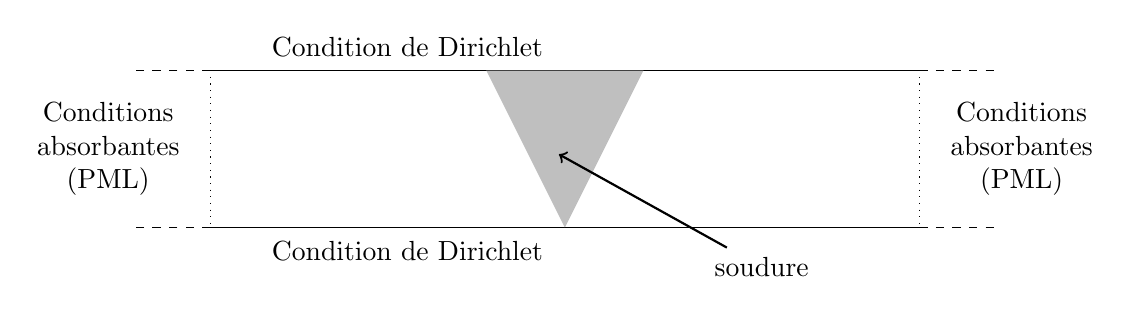
\begin{tikzpicture}
		\draw (0,0) -- (9,0) ;
		\draw (0,-2) -- (9,-2) ;
		\filldraw [fill=gray, fill opacity=0.5, draw=none] (3.5,0) -- (4.5,-2) -- (5.5,0)  ;
		\node (centre) at (4.3,-1) {};
		\node (soudure) at (7,-2.5) {soudure};
		\draw[<-,thick] (centre) -- (soudure);
		\node (fs) [align=left] at (2.5,0.3) {Condition de Dirichlet}	;
		\node (fs2)[align=left] at (2.5,-2.3) {Condition de Dirichlet};
		\draw[dotted] (0,0) -- (0,-2);
		\draw[dotted] (9,0) -- (9,-2);
		\node (g) [align=center] at (-1.3,-1) {Conditions \\ absorbantes \\ (PML)};
		\node (d) [align=center] at (10.3	,-1	) {Conditions \\ absorbantes \\ (PML)};
		\draw[dashed] (0,0) -- (-1,0);
		\draw[dashed] (0,-2) -- (-1,-2);
		\draw[dashed] (9,0) -- (10,0);
		\draw[dashed] (9,-2) -- (10,-2);
	\end{tikzpicture}
	\caption{Représentation des deux types de conditions limites du modèle de soudure 2D.\label{BC}}
\end{figure}

\todo[inline]{Questions : qu'est-ce qui est fait en fréquence, qu'est qui est fait en temps (modèle, inversion) ?}

Le problème peut-être résolu dans le domaine temporel ou dans le domaine fréquentiel \citep{vigh_2008}. Le domaine temporel laisse la possibilité d'effectuer une sélection des arrivées d'ondes par fenêtrage temporel mais présente une plus forte susceptibilité au phénomène de saut de phase (décrit dans le paragraphe ????).  De plus, la résolution par différences finies dans le domaine temporel impose un critère de stabilité Courant-Friedrichs-Lewy (CFL) qui peut-être contraignant, surtout en 3D. Dans le domaine fréquentiel, l'équation d'onde étant réduite à un système d'équations linéaires, il est possible d'utiliser des méthodes de résolution directe du type décomposition LU bien qu'en pratique, les performances de ces méthodes soient limitées pour des problèmes comportant un grand nombre d'inconnues.  Les principaux avantages d'une résolution du problème direct dans le domaine fréquentiel sont donc d'intégrer facilement les phénomènes d'atténuation et de permettre une sélection fine des fréquences d'intérêt. \\~\\







\section{Problème inverse}

Le problème inverse est un problème d'optimisation locale visant à réduire l'écart entre les données observées $\bm{d}_{obs}$ et les données calculées $\bm{d}_{cal}(\bm{m})$ pour chaque couple source-récepteur, en ajustant le modèle constitué de M paramètres $\bm{m}$. L'idée est donc de minimiser la norme au sens des moindres carrés de la différence $\bm{d}_{obs}-\bm{d}_{cal}(\bm{m})$ définie comme suit : 
\begin{equation}
	C(\bm{m})=\frac{1}{2}||\bm{d}_{obs}-\bm{d}_{cal}(\bm{m})||^{2}\text{.}
	\label{norm}
\end{equation}
 Le minimum de cette fonction de coût est atteint lorsque la dérivée par rapport aux paramètres du modèle s'annule. Un développement de Taylor au second ordre de $C(\bm{m}+ \bm{\Delta m})$ permet d'écrire : 
 \begin{equation}
 	\frac{\dd C(\bm{m}+\bm{\Delta m})}{\dd m_{i}}= \frac{\dd C(\bm{m})}{\dd m_{i}} + \displaystyle\sum_{j}^{M} \frac{\dd^{2} C(\bm{m})}{\dd m_{j} \dd m_{i}}\Delta m_{j}\text{.}
 \end{equation}
Les termes d'ordres plus élevés sont nuls si le problème direct est linéaire. Le minimum de la fonction de coût est alors atteint en une seule itération en annulant la dérivée : 
\begin{equation}
	\frac{\dd C(\bm{m}+\bm{\Delta m})}{\dd m_{i}} = 0 ~~~~~\Leftrightarrow ~~~~~ \Delta m _{j} = -\left( \frac{\dd ^{2} C(\bm{m})}{\dd m_{j} \dd m_{i} }\right)^{-1} \frac{\dd C (\bm{m})}{\dd m_{i}} \text{.}
\end{equation}
En FWI, le problème inverse n'étant pas linéaire, cette inversion est réalisée sur plusieurs itérations.\\
La direction de descente est donc donnée par le gradient et la dérivée seconde (hessien) donne la courbure de la fonction de coût.\\



\subsection{Calcul du gradient}

D'après l'expression de la norme~\ref{norm}, sa dérivée par rapport aux paramètres $\bm{m}$ (le gradient) est donc : 
\begin{equation}
	 \frac{\dd C (\bm{m})}{\dd m_{i}} = -\tr{\left( \frac{\dd \bm{d}_{cal}(\bm{m}) }{\dd m_{i}} \right)} ( \bm{d}_{obs} - \bm{d}_{cal}(\bm{m})) \text{.}
	 \label{eq_grad}
\end{equation}\\



Le problème direct décrit au paragraphe précédent~(\ref{pd_dir}) peut se mettre sous la forme :
\begin{equation}
	\bm{A}(\bm{m},\bm{r},\xi)\bm{d}_{cal}(\bm{m},\bm{r},\xi)=\bm{s}(\bm{r},\xi)\text{,}
	\label{eq_pb_dir}
\end{equation}

où $\bm{r}$ est la variable d'espace et $\xi$ est le temps ou la fréquence. $\bm{A}$ est un opérateur correspondant à l'équation d'onde et $\bm{s}$ est le terme source. Notons que le vecteur de données $\bm{d}_{cal}$ a une longueur égale au nombre de récepteur et doit donc être étendu de façon a avoir la même longueur que l'espace du problème direct. La dérivée de l'équation~\ref{eq_pb_dir} par rapport à $\bm{m}$ s'écrit : 
\begin{equation}
	\bm{A} \frac{\dd \bm{d}_{cal}(\bm{m})}{\dd m_{i}} + \frac{\dd A}{\dd m_{i}}\bm{d}_{cal}(\bm{m}) = \bm{0} \text{.}
\end{equation}

On a donc : 
\begin{equation}
	\tr{\left( \frac{\dd \bm{d}_{cal}(\bm{m})}{\dd \bm{m}}  \right)} = - \tr{\bm{d}_{cal}(\bm{m})} \tr{\left( \frac{\dd \bm{A}}{\dd \bm{m}} \right)} \tr{A^{-1}}
	\label{sub}
\end{equation} 	

Finalement, en reportant cette expression dans l'équation~\ref{eq_grad}, on obtient l'expression du gradient : 
\begin{equation}
	 \frac{\dd C (\bm{m})}{\dd m_{i}} = \tr{\bm{d}_{cal}(\bm{m})}  \tr{\left( \frac{\dd \bm{A}}{\dd m_{i}}\right)} \tr{\bm{A}} (\bm{d}_{obs} - \bm{d}_{cal}(\bm{m}))^* = \tr{\bm{d}_{cal}(\bm{m})} \tr{\left( \frac{\dd \bm{A}}{\dd m_{i}}\right)} \lambda^*
\end{equation}
\todo[inline]{conjugué de $\Delta d $ ? p.95 These Romain}

Le champ $\lambda^*$ correspond donc à la rétropopagation des résidus $( \bm{d}_{obs} - \bm{d}_{cal}(\bm{m}))^*$. L'opérateur conjugué $^*$ indique une propagation en temps inverse, ce qui permet, comme en retournement temporel \citep{prada_2002}, une focalisation sur les éléments diffractant absents du modèle initial. Cette expression du gradient peut également être obtenu par le formalise de l'état adjoint \citep{plessix}.\\
\todo[inline]{quid de dA/dm ? Diagramme de rayonnement ?}

La substitution~\ref{sub} permet d'éviter le calcul de la matrice de sensibilité $\tr{\left( \frac{\dd \bm{d}_{cal}(\bm{m}) }{\dd m_{i}} \right)}$ . Le calcul du gradient découle donc du calcul de deux problèmes directs : 
\begin{equation*}
	\bm{A}(\bm{m})\bm{d}_{cal}(\bm{m})=\bm{s} ~~~~~~~\text{et}~~~~~~~\bm{A}(\bm{m}) \lambda^*(\bm{m})=( \bm{d}_{obs} - \bm{d}_{cal}(\bm{m}))^*
\end{equation*}

\subsection{Calcul du hessien}

La méthode d'optimisation choisie pour la FWI est une méthode quasi-Newton qui propose d'utiliser une version approximée de l'inverse du hessien, calculée à partir de valeurs précédentes du gradient.  \cite{brossier_2009} montrent que cette méthode, développée avec l'algorithme L-BFGS, est plus performante que la méthode du gradient conjugué préconditionné en terme de convergence. 

\subsection{Régularisation}

Le problème étant mal-posé, il est nécessaire de limiter les artefacts haute-fréquences venant perturber $\bm{\Delta m}$. Pour cela, il est possible d'ajouter un terme de pondération à la fonction de coût qui permet de lisser le modèle. Ce lissage peut aussi être directement appliqué à $\bm{\Delta m}$ sous forme de filtre spatial adapté à la longueur d'onde correspondant à la fréquence d'inversion.

\section{Problématiques liées à l'inversion}

\subsection{Choix du modèle initial}
Afin d'assurer une convergence vers le minimum global, il est nécessaire que le modèle initial se situe dans le bassin d'attraction de la fonctionnelle. Pour cela, il faut s'assurer que le modèle soit cinématiquement acceptable en levant l’ambiguïté sur la phase. Les données temporelles issues de ce modèle doivent donc avoir un retard de moins d'une demi-longueur d'onde par rapport aux données observées vraies. Si cette condition n'est pas respectée, l'algorithme ne permettra pas un bon réajustement des phases et convergera vers un minimum local (cf~\ref{ambig_phase}).

\begin{figure}[!h]
	\centering
	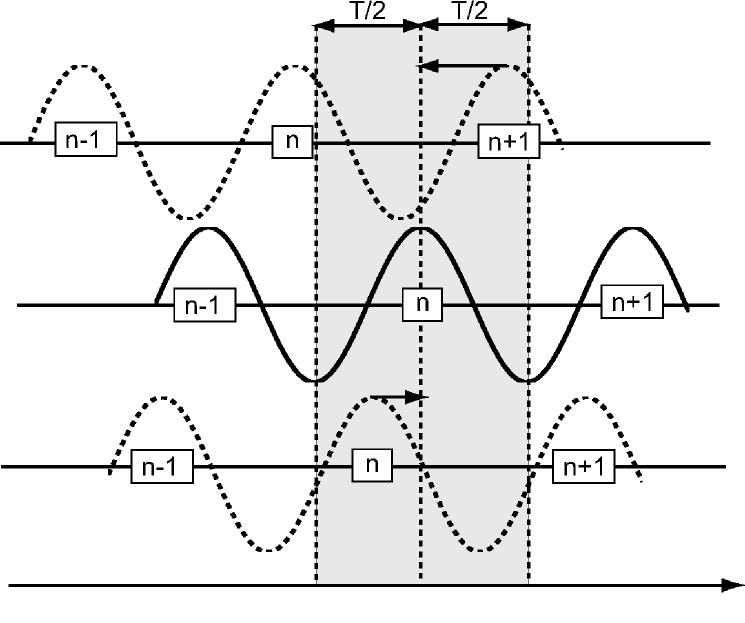
\includegraphics[scale=0.8]{img/ambig_phase.png}
	\caption{Illustration de l'ambiguïté sur la phase (extraite de \cite{brossier_these}). En haut, le déphasage est supérieur à $T/2$, les arches sont mal ajustées. En bas, le déphasage est inférieur à $T/2$, les phases sont bien ajustées. \label{ambig_phase}}
\end{figure}

À défaut de disposer à un modèle initial cinématiquement acceptable, il est possible de d'appliquer un ensemble de stratégies permettant de limiter ces artefacts : introduire progressivement les sources ou récepteurs les plus éloignés, rallonger progressivement les temps d'acquisition, et inverser prioritairement les données basses fréquences.


En sismologie, une image issue de tomographie peut fournir un modèle initial assez précis. Dans cette étude, on considère que peu d'informations sont connues sur les paramètres élastiques de la soudure et le modèle initial choisi est uniforme (cf chapitre~\ref{applications}).


\subsection{Inversion multi-paramètres}
\todo{Passer cette section dans les applications ?}
 
L'inversion multi-paramètres impliques plus de degrés de liberté dans le problème et rend donc l'inversion plus difficile. De plus, ces paramètres peuvent avoir des effets couplés ou non de différentes natures (cinématique ou dynamique) et de différentes amplitudes sur les données. Il faut donc choisir les paramètres à inverser de manière à ce qu'ils décrivent au mieux (de manière complémentaire) les propriétés du milieu à imager. Par exemple, les paramètres de vitesse influencent le champ en terme de temps de vol, tandis que la densité ou l'impédance jouent davantage sur l'amplitude du champ.\\

À chaque ensemble de paramètres est associé un diagramme de rayonnement lié à l'expression de leur différentielle~\citep{forgues}. Ajouté à l'illumination restreinte  par le système d'acquisition, ce rayonnement peut filtrer le spectre en nombre d'onde du milieu reconstitué. Quelques exemples de diagrammes de rayonnement sont présentés en figure~\ref{rayonnement}, où $\kappa$ est le module d'incompressibilité, $\rho$ est la densité, $v_{p}$ est la vitesse des ondes longitudinales se propageant suivant $z$ et $I_{p}$ est l'impédance, tels que : 
\begin{equation*}
	I_{p}=\sqrt{\kappa \rho}~~~~~\text{et}~~~~~\kappa=\rho v_{p}\text{.}
\end{equation*}
Ces diagrammes correspondent au rayonnement des paramètres acoustiques dans un milieu isotrope. En milieu anisotrope, ces diagrammes sont plus difficiles à estimer analytiquement et nécessite une bonne connaissance de l'anisotropie du milieu.

\begin{figure}[!h]
	\centering
	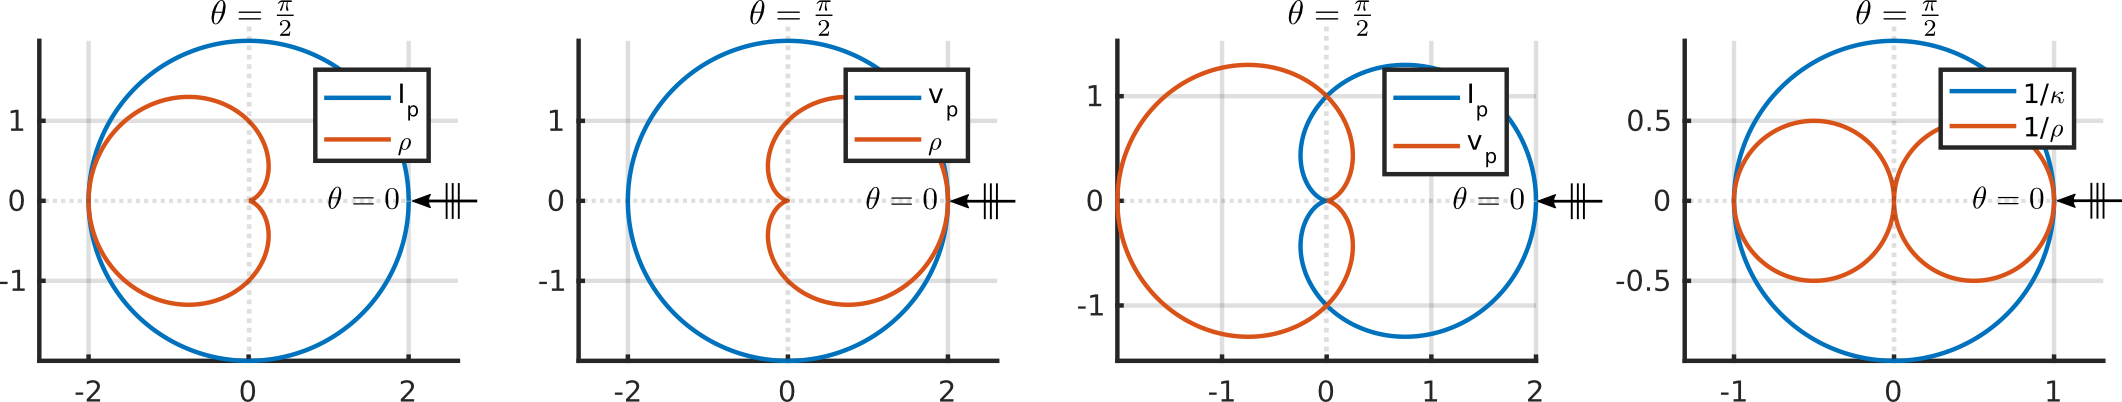
\includegraphics[scale=0.7]{img/rayonnement.png}
	\caption{Diagrammes de rayonnement pour différentes paramétrisations d'un milieu acoustique (amplitudes relatives) tracés d'après \cite{forgues}.\label{rayonnement}}
\end{figure}
%forgues : p.156

\subsection{Estimation de la source}
Pour que les données calculées puissent être comparées aux données observées, il est nécessaire que les termes sources à l'origine des deux champs soit semblables. Ce terme source est linéairement lié au champ (cf équation~\ref{eq_pb_dir}) et il peut donc être calculé par la résolution d'un problème linéaire \citep{pratt_99} dont la solution est : 
$$ s=\frac{\tr{\bm{d}_{cal}(\bm{m})^{*}}\bm{d}_{obs}^{*}}{\bm{d}_{cal}(\tr{\bm{m})^{*}}\bm{d}_{cal}(\bm{m})^{*}}\text{.}$$



\section{Applications en géophysique}

Dans cette section, on se propose de présenter un exemple d'application de la FWI à des données sismologiques dans le cadre de la prospection pétrolière. Dans ce domaine, les mesures étant rares et coûteuses, l'exploitation des données doit être efficace en terme de qualité d'image. C'est pourquoi une méthode comme la FWI y est adaptée, bien qu'elle nécessite beaucoup de ressource informatique.\\
Les images de la figure~\ref{valhall} sont issues des mesures en fond d'océan (Ocean Bottom Cable) par hydrophones.

\todo[inline]{à compléter à partir de l'abstract Sirgue 2009}

\begin{figure}[!h]
    \centering
    \begin{subfigure}[b]{0.4\textwidth}
        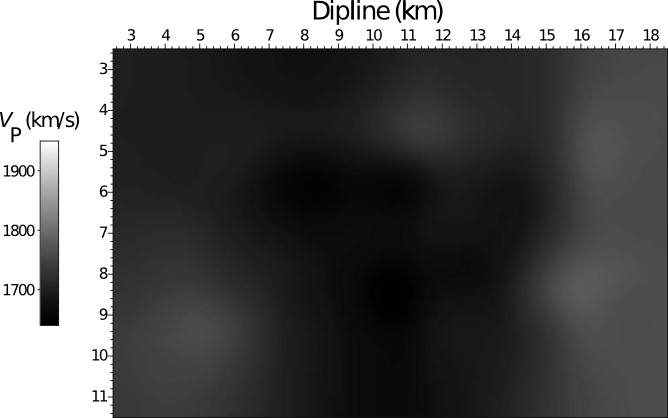
\includegraphics[width=\textwidth]{img/geophy1.png}
        \caption{Par tomographie en réflexion. Coupe à 150 m de profondeur.}
        \label{}
    \end{subfigure}
    \begin{subfigure}[b]{0.4\textwidth}
        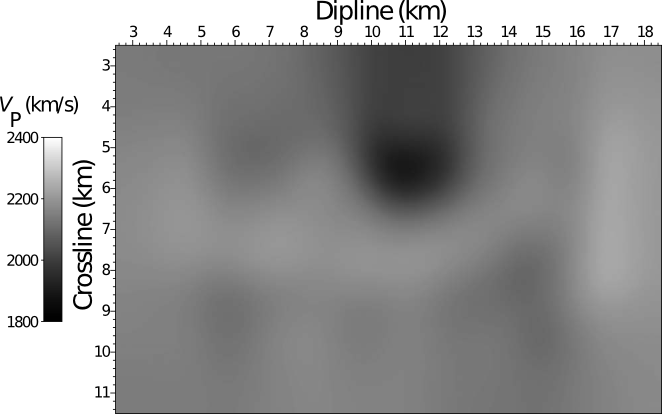
\includegraphics[width=\textwidth]{img/geophy2.png}
        \caption{Par tomographie en réflexion. Coupe à plus de 1000 m de profondeur.}
        \label{}
    \end{subfigure}\\
    \begin{subfigure}[b]{0.4\textwidth}
        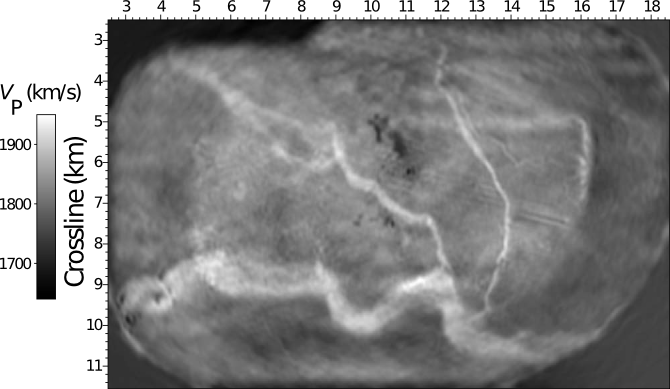
\includegraphics[width=\textwidth]{img/geophy3.png}
        \caption{Par FWI. Coupe à 150 m de profondeur.}
        \label{}
    \end{subfigure}
    \begin{subfigure}[b]{0.4\textwidth}
        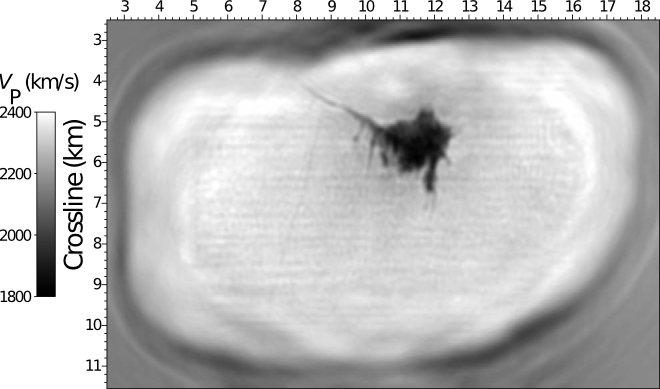
\includegraphics[width=\textwidth]{img/geophy4.png}
        \caption{Par FWI. Coupe à plus de 1000 m de profondeur.}
        \label{}
    \end{subfigure}
    \caption{Images des vitesses dans le champ de Valhall.\label{valhall}}
\end{figure} 
    \todo[inline]{champ ?}

De manière très semblable, imagerie médicale du module d'élasticité \citep{oberai_03,oberai_04} par la méthode de l'adjoint et à des ondes électromagnétiques, rayon X : natterer ?

\section{application au cnd de soudure : les problématiques}

-guide d'onde
-acquisition en surface seulement, et problématique de la soudure bombée
-anisotropie (cf image soudure) forte, qui touche not. les ondes S.
-acquisition horizontale pas idéale pour inverser la vitesse horizontale (car petits offsets et peu de courbure de rayon comme en géophys) (discuter le choix des paramètres à inverser compte-tenu de la configuration)
-sources et récepteurs mobiles 
-geophysique, dispositif de surface, donc on ne considère que les diffractions rayonnant vers la surface (soit angle de diffraction de max 180°)(Forgues, pages 160). En CND, on illumine des deux côté


%\begin{figure}
%	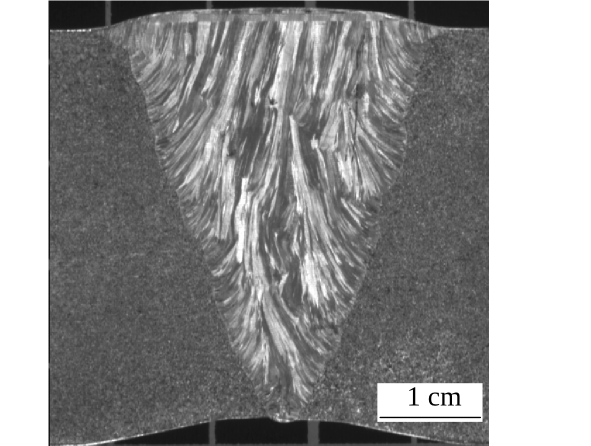
\includegraphics[height=5cm]{./img/soudure1.png}
%	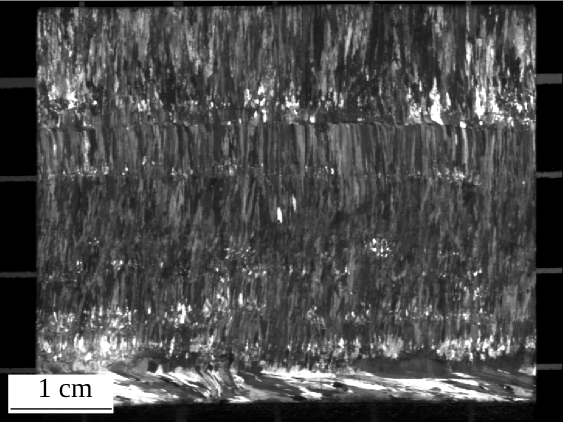
\includegraphics[height=5cm]{./img/soudure2.png}
%	\caption{Macrographie d'une soudure industrielle en acier inoxydable en acier austénitique \citep{chassignole}. À gauche : coupe dans le plan $(x,z)$, à droite : coupe dans le plan $(x,y)$.}
%\end{figure}

grains colonnaires

p91 potel bruneau : données "d'aspect limité" : il n'es tpas possible de tourner autour de l'obstace. On colpense la perte d'info en réalisant les mesures sur plusieurs freq et possibilité de déplacer capteur.




\subsection{sensibilité au bruit ?}

\todo[inline]{Les impasses volontairement faites : \\
	- détail de la discrétisation différences finies / détail des calculs FEM\\	
}


\todo[inline]{born approx}
